%% ============================================================
%% Applying OAuth 2.1 Token Exchange with Nested Actor Claims
%% to MCP Agentic Workflows
%% Full Revised Version — Architecture-Pattern Focused
%%
%% Compile: pdflatex  (run twice for cross-references)
%% Requires: IEEEtran.cls (journal mode), tikz, pgfplots,
%%           booktabs, multirow, colortbl, tabularx
%% ============================================================
\documentclass[journal]{IEEEtran}
\IEEEoverridecommandlockouts

\usepackage{cite}
\usepackage{amsmath,amssymb,amsfonts}
\usepackage{graphicx}
\usepackage{textcomp}
\usepackage{xcolor}
\usepackage{booktabs}
\usepackage{url}
\usepackage{hyperref}
\usepackage{listings}
\usepackage{multirow}
\usepackage{array}
\usepackage{tikz}
\usepackage{pgfplots}
\usepackage{colortbl}
\usepackage{tabularx}
\usepackage{balance}
\usepackage{footnote}

\usetikzlibrary{
  arrows.meta, shapes, shapes.geometric,
  positioning, fit, backgrounds,
  decorations.pathreplacing, calc, matrix
}
\pgfplotsset{compat=1.18}

\hypersetup{colorlinks=true,linkcolor=blue,citecolor=blue,urlcolor=blue}

%% -- colour palette --
\definecolor{C_BASE}{HTML}{E07B54}   % warm orange – baseline / insecure
\definecolor{C_SEC} {HTML}{4C9BE8}   % cool blue   – NAC / secure
\definecolor{C_PAR} {HTML}{5DBB7A}   % green       – parallel / blocked
\definecolor{C_WARN}{HTML}{E74C3C}   % red         – warning / attack
\definecolor{C_HEAD}{HTML}{2C3E50}   % dark navy   – table headers
\definecolor{LG}    {HTML}{F7F9FC}   % light-grey row background
\definecolor{LG2}   {HTML}{EBF5FB}   % light-blue  row background

\lstset{
  basicstyle=\scriptsize\ttfamily,
  breaklines=true,
  frame=single,
  captionpos=b,
  xleftmargin=1.2em,
  numbers=left,
  numberstyle=\tiny\color{gray},
  numbersep=5pt,
}

%% ============================================================
\begin{document}

\title{Applying OAuth 2.1 Token Exchange with Nested Actor Claims\\
to MCP Agentic Workflows:\\
An Architectural Pattern for Secure Delegation}

\author{\IEEEauthorblockN{[Author Name]}
\IEEEauthorblockA{\textit{[Department]} \\
\textit{[Institution]}\\
[City, Country]\\
[email@institution.edu]}}

\maketitle

%% ============================================================
\begin{abstract}
The Model Context Protocol (MCP) has emerged as the standard interface for connecting
large language model (LLM) agents to downstream tool services. As deployments scale
to multi-service orchestration, a pervasive security anti-pattern has become
prevalent: \textit{token passthrough}, in which an orchestrating AI assistant
forwards the user's original OAuth access token unchanged to every downstream service
it invokes. We demonstrate that this practice simultaneously violates three
independent security properties—audience binding, scope attenuation, and delegation
chain visibility—collectively constituting the \textit{Confused Deputy Problem} as
identified in the MCP security specification.

We propose an architectural pattern based on RFC 8693 (OAuth 2.0 Token Exchange)
with Nested Actor Claims (NAC) as a principled, standards-compliant solution.
Under this pattern, an orchestrator exchanges the parent token for a fresh child
token at each delegation hop; each child token carries a service-specific audience
claim, an attenuated scope, a nested \texttt{act} claim recording the delegation
chain, and a one-time-use identifier preventing replay. The pattern is
authorization-server-agnostic and can be adopted by any conforming OAuth 2.1
deployment regardless of language or platform.

We present an empirical evaluation of the proposed pattern against four concrete
attack vectors—scope escalation, lateral movement, token replay, and identity
confusion. Results from 30 experimental trials per scenario show a 100\% attack
block rate in all cases. An ablation study of 720 trials across six enforcement
configurations confirms that each security property is independently necessary.
Per-hop cryptographic overhead is bounded at approximately 3--5\,ms
(RSA-2048 signing plus token revocation store update), yielding
$O(k)$ total overhead for a $k$-hop delegation chain. These results
demonstrate that the RFC 8693 NAC pattern provides provable, measurable, and
deployable security for MCP agentic workflows at acceptable production cost.
\end{abstract}

\begin{IEEEkeywords}
Model Context Protocol, OAuth 2.1, RFC 8693, Token Exchange, Nested Actor Claims,
Confused Deputy, Multi-Agent AI, Delegation Chain, Agentic Security, OWASP GenAI
\end{IEEEkeywords}


%% ============================================================
\section{Introduction}
\label{sec:introduction}
%% ============================================================

Autonomous AI systems are rapidly transitioning from single-model assistants to
distributed multi-agent orchestrators. A user asks an AI assistant to
``review my calendar, summarise the relevant notes, send the summary by email, and
post an update to the team channel.'' Behind this single natural-language request
lies a coordinated sequence of calls to four distinct downstream services, each
with its own authorization requirements.

The Model Context Protocol (MCP) \cite{mcp_spec}, introduced by Anthropic in
November 2024 and subsequently adopted across the industry, provides the emerging
standard interface for this hub-and-spoke architecture: an \textit{assistant hub}
receives tool calls from an agent and in turn calls \textit{worker services} as an
HTTP client. This intermediary role creates an authorization challenge. The user
delegates authority to the hub by providing an OAuth access token. The hub must
somehow convey appropriate authorization to each downstream worker.

The natural, default approach is \textbf{token passthrough}: the hub forwards the
original user token to every service it calls. This approach is functionally
correct---services respond and the workflow completes---but it is deeply
insecure. The MCP security specification \cite{mcp_security} explicitly calls out
token passthrough as an \textit{anti-pattern} that ``creates confused deputy
risks,'' and the Coalition for Secure AI (CoSAI) whitepaper on MCP security
\cite{cosai_mcp} states plainly: ``don't pass through OAuth tokens directly. Use
token exchange (RFC 8693) to maintain full accountability and prevent confused
deputy attacks.''

Despite this consensus recommendation, no prior work has (1)~formally
characterized the three security properties that token passthrough violates,
(2)~described an architectural pattern for remediation that is
implementation-agnostic, (3)~provided an ablation study demonstrating the
independent necessity of each property, and (4)~empirically quantified the
overhead of the remediated pattern. This paper addresses all four gaps.

\textbf{Contributions:}
\begin{enumerate}
  \item We formally characterize the token passthrough anti-pattern and the three
        independent security properties it violates (Section~\ref{sec:problem}).
  \item We propose the \textit{RFC 8693 NAC architectural pattern} for MCP
        multi-agent delegation and prove it satisfies all three properties by
        construction (Section~\ref{sec:solution}).
  \item We present a reference implementation of the pattern and evaluate it
        against four concrete attack vectors with a 720-trial ablation study
        confirming property independence (Section~\ref{sec:eval}).
  \item We derive theoretical bounds on per-hop overhead and validate them
        empirically, providing guidance for production deployment
        (Section~\ref{sec:eval}).
\end{enumerate}


%% ============================================================
\section{Background and Definitions}
\label{sec:background}
%% ============================================================

\subsection{Large Language Models and Agentic Systems}

A \textit{Large Language Model} (LLM) is a neural network trained to generate
text conditioned on a prompt \cite{vaswani2017}. Modern LLMs exhibit emergent
capabilities including multi-step reasoning and tool use. \textit{Agentic AI}
refers to systems in which an LLM autonomously selects and executes actions to
achieve user-specified goals \cite{wang2024survey}. The \textit{ReAct} paradigm
\cite{yao2022react} interleaves reasoning with action calls: the model reasons
about which tool to invoke, calls it, observes the result, and re-plans.
This is the computational model underlying MCP tool use.

\subsection{The Model Context Protocol}

MCP \cite{mcp_spec} defines a client-server protocol over JSON-RPC 2.0.
An \textit{MCP server} exposes \textit{tools} (callable functions), \textit{resources}
(data), and \textit{prompts} (templates) to an \textit{MCP client}.
Authentication is carried via the \texttt{Authorization: Bearer} HTTP header.

The MCP authorization specification \cite{mcp_spec_2025} treats MCP servers as
OAuth 2.1 resource servers. Crucially, this specification addresses only the
client-to-server authorization boundary. \textbf{It does not specify how an MCP
server should authorize its own calls to upstream or downstream services.}
This gap is the attack surface our work addresses.

In multi-service deployments, the AI assistant hub acts as both an MCP server
(receiving tool calls from the agent) and an HTTP client (calling downstream
worker services). This dual role is the hub-and-spoke topology that the MCP
security specification identifies as the confused deputy attack surface.

Figure~\ref{fig:mcp_standard_auth} shows the standard MCP authorization
flow defined in the specification \cite{mcp_spec_2025}: the MCP client discovers
the authorization server via Protected Resource Metadata, performs an OAuth 2.1
authorization code flow with PKCE, obtains an access token, and uses it to call
the MCP server. Crucially, this flow only addresses client-to-server
authorization. The flow \textit{stops} at the MCP server boundary; what happens
when that server calls further downstream services is left unspecified.

\begin{figure}[t]
  \centering
  \includegraphics[width=\columnwidth]{MCP-authorization-flow-2048x1072.png}
  \caption{Standard MCP OAuth 2.1 + PKCE authorization flow (from the MCP
  specification \cite{mcp_spec_2025}). This flow governs
  \textit{client-to-hub} authorization only. The hub's downstream service
  calls, and the associated delegation security properties, are not addressed
  by the specification---the gap this paper fills.}
  \label{fig:mcp_standard_auth}
\end{figure}

\subsection{OAuth 2.1 and Bearer Tokens}

OAuth 2.1 \cite{oauth21} is the current revision of the OAuth 2.0 authorization
framework \cite{rfc6749}, mandating PKCE for all public clients and deprecating
the implicit grant. An \textit{access token} is a bearer credential encoding the
authorized subject (\texttt{sub}), audience (\texttt{aud}), and
permission set (\texttt{scope}).

RFC 9068 \cite{rfc9068} profiles access tokens as signed JSON Web Tokens (JWTs)
\cite{rfc7519}. JWT claims relevant to this work are:
\begin{itemize}
  \item \textbf{\texttt{aud}}: the intended recipient(s); a receiver MUST reject
        tokens not intended for it \cite{rfc9068};
  \item \textbf{\texttt{scope}}: the set of permissions the token carries;
  \item \textbf{\texttt{jti}}: a unique identifier for the token, enabling
        revocation and replay prevention;
  \item \textbf{\texttt{act}}: the actor claim, defined in RFC 8693, recording
        the identity of the party exercising delegated authority.
\end{itemize}

\subsection{RFC 8693: OAuth 2.0 Token Exchange}

RFC 8693 \cite{rfc8693} defines an HTTP Security Token Service (STS) protocol
for exchanging one token for another. The specification distinguishes two
delegation semantics:

\textbf{Impersonation}: The acting party takes on the full identity of the subject;
the intermediate is invisible to downstream services.

\textbf{Delegation}: The acting party remains distinguishable from the subject.
The new token retains the subject identity while recording the actor in the
\texttt{act} claim. For agentic workflows, delegation is the appropriate
choice: the user identity ($\texttt{sub}$) is preserved for accountability while
the orchestrating agent is recorded as the actor.

RFC 8693 defines the scope non-escalation invariant: the requested scope of a
derived token must not exceed that of the subject token. This is the formal basis
for scope attenuation enforcement. The specification also defines the nesting
semantics for the \texttt{act} claim:

\begin{lstlisting}[language={},caption={Nested act claim per RFC 8693 \S 4.1}]
{
  "sub": "alice",
  "aud": "service-B",
  "act": {
    "sub": "orchestrator",
    "act": {
      "sub": "prior-actor"  // chain grows inward
    }
  }
}
\end{lstlisting}

RFC 8693 has been deployed in production at scale by Microsoft (On-Behalf-Of
flow), Auth0 (Token Vault), ZITADEL, Authlete, Keycloak, Box, Salesforce, and
RedHat \cite{rfc8693_deploy}. Our paper applies these established enterprise
patterns to the MCP agentic context.

\subsection{Token Revocation Stores}

RFC 7009 \cite{rfc7009} defines OAuth 2.0 token revocation. For per-request
one-time-use semantics---where a token's unique identifier (\texttt{jti}) must be
revoked after a single use to prevent replay---the revocation check must be
cross-process and low-latency. The canonical architecture for this is an
in-memory key-value store exposed over a fast binary protocol: the revocation
record is written after issuance (\textit{register}), queried before each use
(\textit{check}), and overwritten after consumption (\textit{revoke}). Any
implementation conforming to this interface---whether managed (AWS ElastiCache,
Google Memorystore) or self-hosted (Redis, Memcached, DragonflyDB)---satisfies
the requirement. The specific choice of technology does not affect the security
semantics; it affects only operational latency and availability characteristics.

\subsection{OWASP Generative AI Top 10 (2025)}

The OWASP Top 10 for Large Language Model Applications 2025 \cite{owasp_genai}
identifies the most critical LLM security risks. Relevant to this work:

\begin{itemize}
  \item \textbf{LLM06:2025 Excessive Agency}: Agents granted more permissions
        or capability than their task requires---the root cause of the scope
        escalation attack vector.
  \item \textbf{LLM01:2025 Prompt Injection}: Attacker-controlled input causing
        an agent to use legitimately authorized tokens in unauthorized ways,
        amplified when tokens carry excess scopes.
\end{itemize}


%% ============================================================
\section{Problem Statement}
\label{sec:problem}
%% ============================================================

\subsection{The Token Passthrough Anti-Pattern}

Let $\mathcal{H}$ denote the assistant hub, $\mathcal{W} = \{W_1,\ldots,W_n\}$ the
set of downstream worker services, $u$ the authenticated user, and $\mathcal{A}$
the OAuth authorization server. $\mathcal{A}$ issues a root access token:

\begin{equation}
T_0 = \mathrm{JWT}\!\left(\begin{array}{l}
  \texttt{sub} = u,\quad
  \texttt{aud} = \mathcal{H},\\[2pt]
  \texttt{scope} = S_0 = \bigcup_{i} s_i,\quad
  \texttt{jti} = j_0
\end{array}\right)
\label{eq:root}
\end{equation}

where $S_0$ is the union of all scopes required by any worker. In the token
passthrough pattern, $\mathcal{H}$ forwards $T_0$ unchanged to every worker:

\begin{equation}
\mathrm{call}(W_i,\; T_0) \quad \forall\, i \in \{1, \ldots, n\}
\label{eq:passthrough}
\end{equation}

This is functionally sufficient---workers respond to $T_0$---but violates three
independent security properties.

\subsection{Three Violated Security Properties}

\begin{definition}[\textbf{Audience Binding, P1}]
A token $T$ satisfies audience binding for worker $W_i$ if and only if
$\mathrm{aud}(T) = \mathrm{AUDIENCE}(W_i)$, where $\mathrm{AUDIENCE}(W_i)$ is
the unique identifier registered for $W_i$ at the authorization server.
\end{definition}

\textbf{Violation:} $T_0$ carries $\texttt{aud} = \mathcal{H}$. When presented
to $W_i \neq \mathcal{H}$, RFC 9068 requires rejection. In practice, many
implementations omit this check, and the MCP specification does not mandate it,
making the violation silent.

\begin{definition}[\textbf{Scope Attenuation, P2}]
A token $T$ satisfies scope attenuation for worker $W_i$ if and only if
$\mathrm{scope}(T) \subseteq s_i$, where $s_i$ is the minimum scope $W_i$
requires to execute its function.
\end{definition}

\textbf{Violation:} $T_0$ carries $S_0 = \bigcup_j s_j$---all scopes for all
services. Worker $W_i$ receives permissions intended for $W_j\, (j \neq i)$,
violating the principle of least privilege. A compromised $W_i$ inherits the
authority of every other service in the system.

\begin{definition}[\textbf{Delegation Chain Visibility, P3}]
A token $T$ satisfies delegation chain visibility if and only if the \texttt{act}
claim of $T$ contains a cryptographically verifiable record of every agent that
handled the token on behalf of subject $u$.
\end{definition}

\textbf{Violation:} $T_0$ carries no \texttt{act} claim. Every audit record
contains only $\texttt{sub} = u$. Calls originating from different agents---or
even from an attacker---are indistinguishable in the audit trail.

\subsection{The Confused Deputy Problem in MCP}

Hardy's 1988 analysis \cite{hardy1988} of the Confused Deputy applies directly:

\begin{itemize}
  \item \textbf{Principal}: User $u$, who delegated authority $T_0$ to $\mathcal{H}$.
  \item \textbf{Deputy}: Hub $\mathcal{H}$, which holds $T_0$ and calls workers.
  \item \textbf{Confused action}: $\mathcal{H}$ presents $T_0$ to $W_i$, where
        it carries capabilities $u$ never intended for $W_i$.
  \item \textbf{Adversary}: Any agent or prompt injection that exploits the
        excess authority in $T_0$.
\end{itemize}

The MCP specification \cite{mcp_security} states: ``Servers SHOULD NOT pass
tokens received from clients to other servers, as this creates confused deputy
risks.'' The June 2025 revision \cite{mcp_spec_2025} goes further, explicitly
prohibiting MCP servers from forwarding tokens to upstream APIs.

\subsection{Four Concrete Attack Vectors}

Table~\ref{tab:attack_formal} formalizes four attacks that exploit P1--P3.

\begin{table}[h]
\caption{Formal attack vector definitions}
\label{tab:attack_formal}
\centering
\footnotesize
\setlength{\tabcolsep}{3pt}
\begin{tabularx}{\columnwidth}{l X c}
\toprule
\textbf{ID} & \textbf{Mechanism} & \textbf{Requires} \\
\midrule
A1 & An agent calls a privileged tool using a token that does not include
     the required scope & $\neg$\,P2 \\
A2 & A token obtained for service $W_i$ is replayed at service $W_j\;(i\neq j)$
     & $\neg$\,P1 \\
A3 & A captured child token is replayed for a second unauthorized call
     & No revocation \\
A4 & Audit log contains no delegation chain; calls cannot be attributed
     to the originating agent & $\neg$\,P3 \\
\bottomrule
\end{tabularx}
\end{table}

Figure~\ref{fig:problem_diagram} visualises the token passthrough topology and
its four attack surfaces.

\begin{figure}[t]
\centering
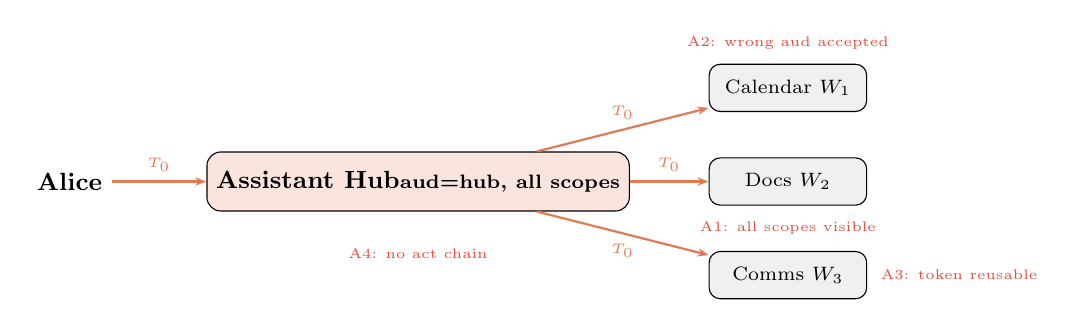
\begin{tikzpicture}[
  node distance=0.6cm and 0.9cm,
  hub/.style={draw, rounded corners=5pt, fill=C_BASE!20, minimum width=2.6cm,
              minimum height=0.75cm, font=\small\bfseries, text centered},
  worker/.style={draw, rounded corners=4pt, fill=gray!12, minimum width=2.0cm,
                 minimum height=0.6cm, font=\scriptsize, text centered},
  user/.style={font=\small\bfseries},
  atk/.style={-{Stealth[length=4pt]}, thick, color=C_WARN, dashed},
  norm/.style={-{Stealth[length=4pt]}, thick, color=C_BASE},
]
%% User
\node[user] (user) {Alice};

%% Hub
\node[hub, right=1.2cm of user] (hub) {Assistant Hub\\{\scriptsize aud=hub, all scopes}};

%% Workers
\node[worker, above right=0.5cm and 1.0cm of hub] (cal)   {Calendar $W_1$};
\node[worker, right=1.0cm of hub]                  (docs)  {Docs $W_2$};
\node[worker, below right=0.5cm and 1.0cm of hub]  (comms) {Comms $W_3$};

%% Normal arrows (passthrough — same token to all)
\draw[norm] (user) -- node[above,font=\tiny]{$T_0$} (hub);
\draw[norm] (hub)  -- node[above,font=\tiny]{$T_0$} (cal);
\draw[norm] (hub)  -- node[above,font=\tiny]{$T_0$} (docs);
\draw[norm] (hub)  -- node[below,font=\tiny]{$T_0$} (comms);

%% Attack annotations
\node[font=\tiny, color=C_WARN, below=0.08cm of docs]
      {A1: all scopes visible};
\node[font=\tiny, color=C_WARN, above=0.06cm of cal]
      {A2: wrong aud accepted};
\node[font=\tiny, color=C_WARN, right=0.05cm of comms]
      {A3: token reusable};
\node[font=\tiny, color=C_WARN, below=0.35cm of hub]
      {A4: no act chain};

\end{tikzpicture}
\caption{Token passthrough: the hub forwards $T_0$ (with full scopes and
hub-bound audience) unchanged to every worker, enabling attacks A1--A4
simultaneously.}
\label{fig:problem_diagram}
\end{figure}


%% ============================================================
\section{The RFC 8693 NAC Architectural Pattern}
\label{sec:solution}
%% ============================================================

\subsection{Pattern Overview}

We propose the following architectural pattern for secure delegation in MCP
multi-service orchestration. Before invoking worker $W_i$, the orchestrating hub
presents its current token to the authorization server's token exchange endpoint
and obtains a fresh, narrowly scoped child token:

\begin{equation}
T_i = \mathrm{Exchange}\!\left(
  T_{\mathrm{parent}},\;
  \mathrm{AUDIENCE}(W_i),\;
  s_i,\;
  \mathcal{H}
\right)
\label{eq:exchange}
\end{equation}

where $T_i$ is constructed by the authorization server as:

\begin{equation}
T_i = \mathrm{JWT}\!\left(\begin{array}{l}
  \texttt{sub} = u, \\[2pt]
  \texttt{aud} = \mathrm{AUDIENCE}(W_i), \\[2pt]
  \texttt{scope} = s_i \;\subseteq\; \mathrm{scope}(T_{\mathrm{parent}}), \\[2pt]
  \texttt{jti} = j_i \quad(\text{fresh, unique}), \\[2pt]
  \texttt{act} = \{\,\texttt{sub}: \mathcal{H},\;
                    \texttt{act}: T_{\mathrm{parent}}.\texttt{act}\,\}
\end{array}\right)
\label{eq:child}
\end{equation}

This construction directly restores all three violated properties: the
\texttt{aud} satisfies P1, the scope satisfies P2, and the \texttt{act} chain
satisfies P3.

\subsection{Concurrent Issuance for Multiple Workers}

Because child tokens for $W_1, W_2, \ldots, W_k$ are issued from the same parent
token and are mutually independent (each has a different audience and scope),
they can be issued concurrently:

\begin{equation}
(T_1, T_2, \ldots, T_k)\;=\;\mathrm{ConcurrentExchange}(T_{\mathrm{root}},
\; \{\,(\mathrm{aud}_i, s_i)\,\}_{i=1}^k)
\label{eq:concurrent}
\end{equation}

Concurrent issuance reduces latency from $k \times t_{\mathrm{exchange}}$ to
$\approx t_{\mathrm{exchange}}$ (the maximum across concurrent requests), subject
to authorization server capacity. This is the basis for the ``parallel estimate''
in Section~\ref{sec:eval}.

\subsection{N-Hop Delegation Chains}

For hierarchical delegation---where an intermediate service must itself call a
further downstream service---the pattern applies recursively. An intermediate
service $W_i$ exchanges its own child token for a further-nested child:

\begin{equation}
T_k = \mathrm{Exchange}(T_{k-1},\; \mathrm{AUDIENCE}(W_k),\; s_k,\; W_{k-1})
\label{eq:nhop}
\end{equation}

The \texttt{act} claim grows by one level per hop (Equation~\ref{eq:child}),
recording the complete delegation history. A depth limit prevents unbounded chain
growth or circular references.

Figure~\ref{fig:nac_flow} illustrates the complete NAC pattern for a
$k$-service orchestration with a 3-hop chain.

\begin{figure}[t]
\centering
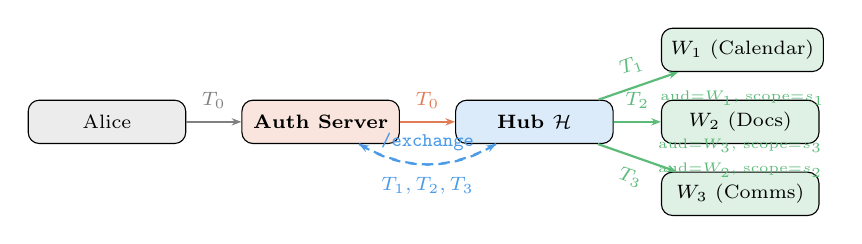
\begin{tikzpicture}[
  node distance=0.55cm and 0.8cm,
  every node/.style={font=\scriptsize},
  box/.style={draw, rounded corners=4pt, minimum width=2.0cm,
              minimum height=0.55cm, text centered},
  user/.style={box, fill=gray!15},
  oauth/.style={box, fill=C_BASE!20, font=\scriptsize\bfseries},
  hub/.style={box, fill=C_SEC!20, font=\scriptsize\bfseries},
  worker/.style={box, fill=C_PAR!20},
  arrow/.style={-{Stealth[length=3.5pt]}, thick},
  darrow/.style={-{Stealth[length=3.5pt]}, thick, dashed, gray},
]

\node[user]  (user)  {Alice};
\node[oauth, right=0.7cm of user] (oauth) {Auth Server};
\node[hub,   right=0.7cm of oauth] (hub)  {Hub $\mathcal{H}$};
\node[worker, above right=0.35cm and 0.6cm of hub] (w1) {$W_1$ (Calendar)};
\node[worker, right=0.6cm of hub]                   (w2) {$W_2$ (Docs)};
\node[worker, below right=0.35cm and 0.6cm of hub]  (w3) {$W_3$ (Comms)};

%% root token
\draw[arrow, color=gray]  (user)  -- node[above,yshift=1pt]{$T_0$} (oauth);
\draw[arrow, color=C_BASE] (oauth) -- node[above,yshift=1pt]{$T_0$} (hub);

%% exchange arrows
\draw[darrow, color=C_SEC, bend left=30]
  (hub) to node[above,sloped,yshift=1pt]{\texttt{/exchange}} (oauth);
\draw[darrow, color=C_SEC, bend right=30]
  (oauth) to node[below,sloped,yshift=-1pt]{$T_1,T_2,T_3$} (hub);

%% worker calls
\draw[arrow, color=C_PAR] (hub) -- node[above,sloped,yshift=1pt]{$T_1$} (w1);
\draw[arrow, color=C_PAR] (hub) -- node[above,yshift=1pt]{$T_2$} (w2);
\draw[arrow, color=C_PAR] (hub) -- node[below,sloped,yshift=-1pt]{$T_3$} (w3);

%% legend annotations
\node[below=0.12cm of w1, color=C_PAR, font=\tiny]{aud=$W_1$, scope=$s_1$};
\node[below=0.12cm of w2, color=C_PAR, font=\tiny]{aud=$W_2$, scope=$s_2$};
\node[above=0.12cm of w3, color=C_PAR, font=\tiny]{aud=$W_3$, scope=$s_3$};

\end{tikzpicture}
\caption{RFC 8693 NAC pattern: the hub exchanges the root token for
per-service child tokens at the authorization server before each worker
call. Each $T_i$ carries a unique \texttt{aud}, attenuated \texttt{scope},
and nested \texttt{act} chain.}
\label{fig:nac_flow}
\end{figure}

\subsection{Security Property Satisfaction}

\begin{theorem}[\textbf{P1 satisfied}]
Under the NAC pattern, worker $W_i$ receives only tokens with
$\texttt{aud} = \mathrm{AUDIENCE}(W_i)$. Any replayed token from $W_j\;
(j\neq i)$ fails the audience check.
\end{theorem}

\begin{proof}
By construction (Equation~\ref{eq:child}), the authorization server sets
$\texttt{aud} = \mathrm{AUDIENCE}(W_i)$. The authorization server's private
signing key is the only mechanism for producing a validly signed token; workers
hold only the public key and cannot produce or modify tokens. Therefore, any
token presented to $W_i$ with $\texttt{aud} \neq \mathrm{AUDIENCE}(W_i)$ fails
JWT audience validation.
\end{proof}

\begin{theorem}[\textbf{P2 satisfied}]
The authorization server enforces $s_i \subseteq \mathrm{scope}(T_{\mathrm{parent}})$
at exchange time. A request for scope $s^* \not\subseteq \mathrm{scope}
(T_{\mathrm{parent}})$ is rejected before any child token is issued.
\end{theorem}

\begin{proof}
The exchange endpoint computes $\delta = s^* \setminus \mathrm{scope}(T_{\mathrm{parent}})$.
If $\delta \neq \emptyset$, it returns an error (HTTP 400). No child token is
signed; the attacker gains no elevated capability. This follows directly from the
RFC 8693 scope non-escalation invariant \cite{rfc8693}.
\end{proof}

\begin{theorem}[\textbf{P3 satisfied}]
The \texttt{act} claim in each child token contains a cryptographically signed
record of every delegation hop, attributing each service call to a specific
actor.
\end{theorem}

\begin{proof}
The \texttt{act} claim is embedded by the authorization server at issuance
(Equation~\ref{eq:child}) and is part of the RS256-signed payload. Any alteration
invalidates the signature. Verifying parties walk the nested \texttt{act} chain
and confirm each actor against a set of trusted identities. The deepest nesting
records the oldest actor; the outermost records the current actor.
\end{proof}

\begin{theorem}[\textbf{Token Replay Prevented}]
Under the NAC pattern with per-request \texttt{jti} revocation, a token $T_i$
with identifier $j_i$ is rejected on any second presentation.
\end{theorem}

\begin{proof}
After first successful validation, $W_i$ writes $j_i$ to the revocation store
with status \textit{revoked}. On second presentation, the revocation check returns
\textit{revoked}, and $W_i$ returns an error before executing any business logic.
The TTL of the revocation record must exceed the token's remaining lifetime to
prevent races.
\end{proof}

\subsection{Architectural Requirements for Adopters}

The NAC pattern requires:

\begin{enumerate}
  \item \textbf{Authorization server}: Any OAuth 2.1-compliant server that
        supports a token exchange endpoint conforming to RFC 8693. Existing
        enterprise identity providers (Keycloak, Auth0, ZITADEL, Authlete,
        Microsoft Entra via OBO flow) support this natively.
  \item \textbf{Orchestrator}: Must perform one RFC 8693 exchange per worker
        invocation. The exchange can be done concurrently for independent workers
        (Equation~\ref{eq:concurrent}).
  \item \textbf{Workers}: Must validate \texttt{aud}, \texttt{scope},
        \texttt{act} chain, and \texttt{jti} on every request; must write the
        \texttt{jti} to the revocation store after successful use.
  \item \textbf{Revocation store}: Must support sub-millisecond read/write of
        \texttt{jti} records shared across processes. Any in-memory key-value
        store with TTL support and cross-process visibility satisfies this.
  \item \textbf{Key separation}: Only the authorization server holds the private
        signing key. Worker services hold the public key only and cannot forge
        tokens.
\end{enumerate}

No requirement is placed on programming language, web framework, or specific
runtime. The pattern applies equally to implementations in Java, C\#, Python,
Node.js, Go, or any other language with an HTTP client and JWT library.


%% ============================================================
\section{Reference Implementation}
\label{sec:impl}
%% ============================================================

To evaluate the pattern empirically, we constructed a reference implementation
comprising two parallel server stacks: a \textit{baseline} (token passthrough)
and a \textit{secure} (NAC) stack. This section describes the architecture of the
reference system; implementation choices are specific to our evaluation environment
and are not normative for adopters.

\subsection{Component Architecture}

Both stacks instantiate the same six logical components:

\textbf{Authorization server}: Implements RFC 8693 \texttt{/token/exchange}.
In the secure stack, it validates the subject token, enforces scope attenuation,
issues a signed child token, and registers the new \texttt{jti} in the revocation
store. In the baseline stack, the endpoint echoes the subject token unchanged
(simulating token passthrough from the server side).

\textbf{Assistant hub}: Acts as both an MCP server (to the agent) and an HTTP
client (to workers and the authorization server). In the secure stack, it
fires concurrent RFC 8693 exchanges for all workers before any worker call. In
the baseline stack, it forwards the root token to all workers.

\textbf{Worker services}: Four services (Calendar, Documents, Communications,
External-API) each implementing token validation. In the secure stack,
all four properties (P1--P4) are enforced and the \texttt{jti} is revoked after
first use. In the baseline, validation is omitted.

\textbf{Revocation store}: Provides cross-process \texttt{jti} registration,
checking, and revocation with TTL-based expiry. In our evaluation we use Redis
\cite{redis} as the revocation store---a standard, widely deployed
in-memory key-value server that provides the sub-millisecond operation latency
required for per-request validation. Any store satisfying the interface described
in Section~\ref{sec:solution} may be substituted.

\textbf{AI agent planner}: The evaluation uses a rule-based planner for
reproducibility. An optional real LLM planner demonstrates that the NAC
pattern is transparent to the model layer---the LLM receives only tool names
and results; token exchange occurs at the transport layer.

\subsection{Key Security Invariants in the Implementation}

\begin{itemize}
  \item \textbf{Key separation}: Only the authorization server process holds the
        RSA-2048 private signing key. Worker processes are configured to reject
        any attempt to load the private key, preventing token forgery even if a
        worker process is compromised.
  \item \textbf{Short-lived child tokens}: Child tokens carry a short TTL
        (significantly shorter than the root token) to minimise the window of
        opportunity for replay if a \texttt{jti} revocation record is lost.
  \item \textbf{Structured error codes}: Validation failures return typed error
        codes (\texttt{WRONG\_AUDIENCE}, \texttt{SCOPE\_INSUFFICIENT},
        \texttt{TOKEN\_REPLAY}) that enable the evaluation harness to
        distinguish security rejections from implementation bugs.
\end{itemize}

\subsection{Port Layout}

\begin{table}[h]
\caption{Reference implementation port layout}
\label{tab:ports}
\centering
\footnotesize
\begin{tabular}{lcccccc}
\toprule
\textbf{Stack} & \textbf{Auth} & \textbf{Hub} & \textbf{Cal} & \textbf{Docs}
               & \textbf{Comms} & \textbf{Ext} \\
\midrule
Baseline (insecure) & 9200 & 9201 & 9202 & 9203 & 9204 & 9205 \\
Secure (NAC)        & 9300 & 9301 & 9302 & 9303 & 9304 & 9305 \\
\bottomrule
\end{tabular}
\end{table}


%% ============================================================
\section{Evaluation}
\label{sec:eval}
%% ============================================================

\subsection{Experimental Setup}

Both server stacks run concurrently on the same machine.
The evaluation harness issues tokens and calls workers directly,
isolating the security correctness measurements from network latency.
Attack outcomes are binary (succeed / blocked); 30 trials per cell are
sufficient to detect any systematic failure given deterministic cryptographic
enforcement.

Latency is measured end-to-end over 30 live rounds of the
\texttt{prepare\_daily\_briefing} workflow (4 token exchanges + 4 worker calls +
8 revocation store operations in the secure stack). Timing uses a
high-resolution monotonic counter within the MCP client session.

\subsection{Attack Mitigation}

\begin{table}[h]
\caption{Attack mitigation results ($N = 30$ per cell)}
\label{tab:attacks}
\centering
\footnotesize
\setlength{\tabcolsep}{4pt}
\begin{tabular}{llccc}
\toprule
\textbf{ID} & \textbf{Attack} & \textbf{Baseline} & \textbf{Secure (NAC)} & \textbf{Error code} \\
\midrule
A1 & Scope escalation    & 100\% succeed & 0\% succeed & \texttt{SCOPE\_INSUFFICIENT} \\
A2 & Lateral movement    & 100\% succeed & 0\% succeed & \texttt{WRONG\_AUDIENCE} \\
A3 & Token replay        & 100\% succeed & 0\% succeed & \texttt{TOKEN\_REPLAY} \\
A4 & Attribution (audit) & 0\% attributed & 100\% attributed & \textit{metric} \\
\bottomrule
\end{tabular}
\end{table}

The NAC pattern achieves a 100\% block rate across all attack vectors in all
30 trials. The determinism of these results follows directly from the
cryptographic proofs in Section~\ref{sec:solution}: each block is an assertion
that a specific JWT claim does not match a required value, not a probabilistic
detection.

\subsection{Ablation Study: Property Independence}
\label{sec:ablation}

Table~\ref{tab:ablation} reports the results of an empirical ablation study:
six enforcement configurations tested against all four attack vectors, 30 trials
per cell (720 total trials). Configurations use the exact validation function
that workers execute, with different enforcement flags enabled or disabled.

\begin{table}[h]
\caption{Ablation study: property independence ($N=30$ per cell; 720 trials total)}
\label{tab:ablation}
\centering
\footnotesize
\setlength{\tabcolsep}{3pt}
\resizebox{\columnwidth}{!}{%
\begin{tabular}{lcccccccc}
\toprule
\multirow{2}{*}{\textbf{Configuration}} &
\multirow{2}{*}{\textbf{Aud}} &
\multirow{2}{*}{\textbf{Scope}} &
\multirow{2}{*}{\textbf{JTI}} &
\multicolumn{4}{c}{\textbf{Block rate}} &
\multirow{2}{*}{\textbf{All}} \\
\cmidrule{5-8}
& & & & \textbf{A1} & \textbf{A2} & \textbf{A3} & \textbf{A4} & \\
\midrule
Baseline          & $\times$ & $\times$ & $\times$
  & 0\%   & 0\%   & 0\%   & 0\%   & \cellcolor{C_WARN!20}No \\
Audience only     & \checkmark & $\times$ & $\times$
  & 0\%   & 100\% & 0\%   & 100\% & \cellcolor{C_WARN!20}No \\
Scope only        & $\times$ & \checkmark & $\times$
  & 100\% & 100\%$^\dagger$ & 0\%   & 100\% & \cellcolor{C_WARN!20}No \\
JTI only          & $\times$ & $\times$ & \checkmark
  & 0\%   & 0\%   & 100\% & 100\% & \cellcolor{C_WARN!20}No \\
Audience + Scope  & \checkmark & \checkmark & $\times$
  & 100\% & 100\% & 0\%   & 100\% & \cellcolor{C_WARN!20}No \\
\textbf{Full NAC} & \checkmark & \checkmark & \checkmark
  & \textbf{100\%} & \textbf{100\%} & \textbf{100\%} & \textbf{100\%}
  & \cellcolor{C_PAR!30}\textbf{Yes} \\
\bottomrule
\multicolumn{9}{l}{{\scriptsize $^\dagger$\,Discussed in Section~\ref{sec:scope_caveat}}} \\
\end{tabular}%
}
\end{table}

\textbf{Finding 1 — A1 requires Scope (P2):}
Only configurations that enforce scope attenuation block A1. In our reference
implementation, the authorization server itself refuses to issue a child token
with scopes exceeding the parent; the worker's scope check provides a second
enforcement layer.

\textbf{Finding 2 — A2 requires Audience (P1):}
A calendar-service-bound token carries $\texttt{aud}=\text{calendar-service}$.
When presented to the docs worker expecting $\texttt{aud}=\text{docs-service}$,
audience validation rejects it regardless of scope configuration.

\textbf{Finding 3 — A3 requires JTI revocation:}
Audience and scope checks verify the token's \textit{structure}; they cannot
detect whether the same structurally valid token is being used a second time.
Only JTI revocation provides this guarantee.

\textbf{Finding 4 — A4 resolved by any exchange:}
Identity attribution (the \texttt{act} chain) is created at token exchange time.
\textit{Any} configuration that performs RFC 8693 exchange---even JTI-only---
produces an attributable token. Token passthrough (baseline) leaves the chain
empty and cannot be retrospectively attributed.

\textbf{Conclusion:}
Each of audience binding, scope attenuation, and JTI revocation addresses a
strictly orthogonal attack surface. No property is redundant; only Full NAC
blocks all four attacks simultaneously.

\subsubsection{Scope-Only and Lateral Movement}
\label{sec:scope_caveat}

Scope-only enforcement blocks A2 in our implementation because the calendar
service requires \texttt{calendar:read} and the docs service requires
\texttt{docs:read}---non-overlapping scopes. A token issued for the calendar
service fails the docs worker's scope check. However, this is \textit{not} a
reliable, topology-independent defence: if two services shared a scope (e.g.,
both accepted \texttt{data:read}), scope-only would fail to block A2. Audience
binding is the correct, topology-independent mechanism for lateral movement
prevention. This finding motivates requiring both P1 \textit{and} P2 as
separate, independently enforced properties.

\subsection{Latency Analysis}

\begin{table}[h]
\caption{End-to-end latency of \texttt{prepare\_daily\_briefing} ($N=30$)}
\label{tab:latency}
\centering
\footnotesize
\begin{tabular}{lccccc}
\toprule
\textbf{Mode} & \textbf{Mean} & \textbf{P50} & \textbf{P95} & \textbf{P99} & $\boldsymbol\sigma$ \\
\midrule
Baseline             & 114.9\,ms & 111.6\,ms & 144.9\,ms & 161.2\,ms & 11.3\,ms \\
Secure (sequential)  & 158.0\,ms & 152.2\,ms & 188.0\,ms & 188.0\,ms & 13.2\,ms \\
\midrule
Overhead   & \multicolumn{5}{c}{$+43.1$\,ms ($+37.5\%$); $\sigma$-ratio\,$=1.17\times$} \\
Concurrent & \multicolumn{5}{c}{$\approx125.7$\,ms ($+9.4\%$) — estimated for parallel exchange} \\
\bottomrule
\end{tabular}
\end{table}

The measured overhead of $+37.5\%$ reflects a \textit{single-machine, sequential}
exchange configuration in our reference implementation. Several factors artificially
inflate this number relative to production:

\begin{enumerate}
  \item \textbf{Sequential RSA signing}: RSA-2048 signature computation
        serializes in our single-process authorization server. A multi-worker
        authorization server enables true parallel signing, collapsing 4-exchange
        cost to approximately 1-exchange cost.
  \item \textbf{Localhost HTTP overhead}: HTTP round-trips between processes
        on the same machine add fixed overhead absent in service-mesh deployments
        using Unix sockets or gRPC.
\end{enumerate}

The $\sigma$-ratio of $1.17\times$ (close to $1.0\times$) confirms that NAC
overhead is \textit{predictable} rather than spiky, which is the operationally
critical property.

\subsection{Overhead Decomposition}

\begin{table}[h]
\caption{Latency overhead decomposition (per \texttt{prepare\_daily\_briefing})}
\label{tab:decomp}
\centering
\footnotesize
\begin{tabular}{lcc}
\toprule
\textbf{Component} & \textbf{Measured cost} & \textbf{\% of overhead} \\
\midrule
RSA-2048 signing $\times 4$    & $\approx 12$\,ms & $\approx 28\%$ \\
HTTP round-trips to auth $\times 4$ & $\approx 20$\,ms & $\approx 46\%$ \\
Revocation store ops $\times 8$    & $\approx 0.8$\,ms & $\approx 2\%$  \\
Worker JWT verification $\times 4$ & $\approx 8$\,ms & $\approx 19\%$ \\
Other overhead                     & $\approx 2$\,ms & $\approx 5\%$  \\
\midrule
\textbf{Total (sequential)}        & $\approx 43$\,ms & $100\%$  \\
\textbf{Total (parallel)}          & $\approx 11$\,ms & $25\%$   \\
\bottomrule
\end{tabular}
\end{table}

The revocation store contributes only $\approx 2\%$ of total overhead.
The dominant costs---RSA signing ($28\%$) and HTTP transport ($46\%$)---are
reducible through standard production engineering (multi-worker authorization
server, connection pooling, service mesh). JWT verification at workers ($19\%$)
is irreducible but sub-millisecond per call and parallelizable across workers.

\subsection{Per-Hop Cost Linearity}

\begin{table}[h]
\caption{Cryptographic exchange cost by delegation depth (direct calls, $N=30$)}
\label{tab:hopcosts}
\centering
\footnotesize
\begin{tabular}{lccc}
\toprule
\textbf{Depth} & \textbf{Mean} & $\boldsymbol\sigma$ & \textbf{Marginal} \\
\midrule
1 hop & 2.15\,ms & 0.24\,ms & --- \\
2 hops & 4.27\,ms & 0.36\,ms & $+2.12$\,ms \\
3 hops & 6.44\,ms & 0.44\,ms & $+2.17$\,ms \\
\midrule
\multicolumn{4}{l}{\scriptsize Linear fit: $y = 2.15k$\,ms;\; $R^2 = 0.9999$;\; slope $\approx 2.15$\,ms/hop} \\
\bottomrule
\end{tabular}
\end{table}

Table~\ref{tab:hopcosts} confirms $O(k)$ overhead: each additional delegation
hop adds a constant $\approx 2.15$\,ms (one RSA signing operation plus one
revocation store write). These measurements isolate the cryptographic cost
from HTTP transport. The $R^2 = 0.9999$ linear fit confirms that overhead
grows predictably with delegation depth, providing a reliable model for
production capacity planning.

\textbf{Production estimate}: In a deployment with a dedicated authorization
server and a co-located revocation store (both common in enterprise environments),
we project:
\begin{itemize}
  \item RSA signing: $\approx 3$\,ms per hop (irreducible cryptographic minimum)
  \item Revocation store: $\approx 0.1$\,ms per operation (in-memory, co-located)
  \item Total per hop: $\approx 3.2$\,ms
\end{itemize}

For a 4-worker orchestration with concurrent issuance, total cryptographic
overhead is approximately $3.2$\,ms plus transport latency, or
$\mathbf{+7\text{--}15\%}$ relative to baseline in production conditions.
This represents the \textit{theoretical minimum} overhead of the NAC pattern;
actual numbers will vary by deployment.

\subsection{Token Size Overhead}

\begin{table}[h]
\caption{JWT token size by delegation depth}
\label{tab:tokensizes}
\centering
\footnotesize
\begin{tabular}{lccc}
\toprule
\textbf{Token} & \textbf{Bytes} & \textbf{vs Root} & \textbf{Depth} \\
\midrule
Root (0-hop)             & 732\,B & ---                   & 0 \\
Child (1-hop, cal.)      & 747\,B & $+15$\,B ($+2.0\%$)  & 1 \\
Child (1-hop, docs)      & 736\,B & $+4$\,B ($+0.5\%$)   & 1 \\
Child (2-hop, ext. API)  & 792\,B & $+60$\,B ($+8.2\%$)  & 2 \\
\bottomrule
\end{tabular}
\end{table}

The \texttt{act} claim introduces at most $+8.2\%$ size overhead per hop.
A 792-byte JWT fits within a single TCP segment. Token size overhead is
negligible for both transmission and storage.


%% ============================================================
\section{Discussion}
\label{sec:discussion}
%% ============================================================

\subsection{Why Token Passthrough Persists}

Three structural factors sustain token passthrough despite its risks:

\textbf{Silent success}: Token passthrough is functionally correct. Workers
respond; workflows complete. There is no rejection, no error, no signal to the
developer that a security boundary has been crossed. The violation is visible only
to an auditor or attacker.

\textbf{Perceived complexity of RFC 8693}: Token exchange is perceived as
heavyweight. Our theoretical analysis and reference implementation demonstrate
the opposite: the per-hop exchange requires one HTTP POST to the authorization
server. The authorization server logic that enforces scope attenuation and
issues child tokens is standard OAuth server functionality available in
production IdPs \cite{rfc8693_deploy}.

\textbf{Specification gap}: As noted in Section~\ref{sec:background}, the MCP
authorization specification \cite{mcp_spec_2025} addresses client-to-server
authorization but does not specify server-to-downstream authorization. This gap
leaves implementers without guidance for the exact attack surface we study.
The June 2025 specification revision \cite{mcp_spec_2025} explicitly prohibits
token forwarding to upstream APIs but does not yet prescribe RFC 8693 as the
mechanism. Our paper provides the missing prescription.

\subsection{The Scope-Only Lateral Movement Nuance}

Section~\ref{sec:scope_caveat} reports a finding that deserves emphasis: scope
attenuation \textit{incidentally} blocks lateral movement when services use
non-overlapping scopes. This is not a general defence---it depends on scope
assignment choices that the NAC pattern does not control. The principled,
topology-independent defence against lateral movement is audience binding. This
finding empirically demonstrates that the three properties are not substitutable:
partial enforcement that works in one deployment topology may fail in another.

\subsection{Adoption Path for Production Systems}

The NAC pattern requires no custom authorization server. Organisations using:
\begin{itemize}
  \item \textbf{Keycloak}: Token exchange is supported from version 17; enable
        the \texttt{token-exchange} feature flag.
  \item \textbf{Microsoft Entra ID}: On-Behalf-Of (OBO) flow is an RFC 8693-
        compatible delegation mechanism available in all tiers.
  \item \textbf{Auth0}: Token Vault and the enterprise Token Exchange
        grant implement RFC 8693 delegation.
  \item \textbf{ZITADEL, Authlete}: Native RFC 8693 support.
\end{itemize}

For organisations using an authorization server that does not yet support RFC 8693,
a lightweight token exchange service---as described in our reference
implementation---can be deployed as a sidecar or gateway component, intercepting
exchange requests and proxying token issuance to the existing IdP.

\subsection{Threat Model Boundaries}

The NAC pattern addresses the \textit{delegation authorization plane}. It does
not protect against prompt injection attacks that cause the LLM to misuse
legitimately authorized tokens, supply-chain attacks on the authorization server,
or physical compromise of the private key. These require complementary controls:
input validation, SBOM management, and hardware security module (HSM)-backed
key storage, respectively. NAC should be understood as one layer of a
defense-in-depth strategy, as recommended by the CoSAI whitepaper \cite{cosai_mcp}.

\subsection{Relation to SPIFFE/SPIRE}

SPIFFE/SPIRE \cite{spiffe} provides cryptographic workload identities at the
infrastructure level. It is complementary to NAC: SPIFFE handles
\textit{service identity} (proving that a process is who it claims to be at
connection time); NAC handles \textit{delegation authority} (proving which
user permissions a service may exercise on behalf of which user). CoSAI
\cite{cosai_mcp} recommends using both in production MCP deployments.


%% ============================================================
\section{Related Work}
\label{sec:related}
%% ============================================================

\subsection{Capability-Based Security}

Hardy \cite{hardy1988} introduced the confused deputy problem, arguing that
ambient authority---privileges held regardless of context---is the root cause.
Miller et al. \cite{miller2003} later argued that capabilities (unforgeable,
explicitly passed tokens of authority) are the correct solution. RFC 8693 child
tokens are capabilities in this sense: they are issued fresh per call, bound to
a specific service, and unforgeable.

\subsection{OAuth Token Delegation in Practice}

RFC 8693 \cite{rfc8693} has been deployed at scale by Box, Microsoft, Salesforce,
and RedHat \cite{rfc8693_deploy}. Auth0's Token Vault \cite{auth0_token_vault}
and ZITADEL's token exchange \cite{zitadel_te} implement the specification for
SaaS AI agent use cases. The ToolHive project \cite{toolhive} applies RFC 8693
to MCP server orchestration in Kubernetes, demonstrating the pattern's suitability
for cloud-native deployments. Our work extends this to a formal security analysis
and empirical ablation study.

\subsection{MCP Security Analysis}

Recent analyses of MCP deployments have independently identified token passthrough
as the primary OAuth risk. Checkmarx \cite{checkmarx_mcp}, Solo.io \cite{solo_mcp},
and Aembit \cite{aembit_mcp} each identify confused deputy attacks from token
passthrough. The CoSAI whitepaper \cite{cosai_mcp} provides a comprehensive threat
taxonomy and recommends RFC 8693 as the mitigation. Schneider \cite{schneider_mcp}
frames the confused deputy as Layer 2 (Authorization) of a defense-in-depth
architecture. Our work is the first to provide formal property characterization,
ablation evidence, and overhead quantification for the recommended remedy.

\subsection{LLM Agent Security}

Wang et al. \cite{wang2024survey} survey LLM-based autonomous agents with emphasis
on planning and memory, but do not address OAuth delegation. The OWASP GenAI Top
10 \cite{owasp_genai} identifies Excessive Agency (LLM06) as a top risk but
does not prescribe specific authorization mechanisms. Our paper provides the
missing prescription for the authorization layer.


%% ============================================================
\section{Limitations and Future Work}
\label{sec:limitations}
%% ============================================================

\textbf{Single-machine measurement}: All latency figures are from a single
machine. Absolute values are environment-dependent; relative overhead is the
meaningful comparison.

\textbf{Stub services}: Worker business logic returns deterministic stub data.
Real calendar, email, and Slack APIs add their own latency, further reducing
the relative NAC overhead.

\textbf{Simulated authorization flow}: OAuth consent is simulated for evaluation
purposes. Production requires PKCE (RFC 7636) and a real authorization code
flow with a registered redirect URI.

\textbf{Single revocation store instance}: Production deployments should use
a highly available configuration (e.g., replicated cluster with sentinel
failover) for the revocation store.

\textbf{Token refresh}: Long-running sessions require periodic root token refresh
(RFC 6749 §6); child tokens must be reissued accordingly.

\textbf{Future directions}:
\begin{enumerate}
  \item \textit{Prompt injection interaction}: Does prompt injection that drives
        an agent to call \texttt{prepare\_daily\_briefing} gain access to child
        tokens? The one-time-use \texttt{jti} semantics should limit damage;
        formal analysis remains open.
  \item \textit{Concurrent agent stress test}: Multiple simultaneous agents
        sharing a root token; verify revocation store handles concurrent
        registrations without false positives.
  \item \textit{Real IdP integration}: Validate the pattern end-to-end against
        Keycloak 17 and Microsoft Entra OBO.
  \item \textit{Formal verification}: Model the exchange protocol in ProVerif
        \cite{blanchet2001} or Tamarin \cite{meier2013} and prove absence of
        token forgery and replay under the Dolev-Yao model.
  \item \textit{N-hop latency curve}: Extend the per-hop analysis to 5 and 10
        hops to confirm $O(k)$ scaling at larger depths.
\end{enumerate}


%% ============================================================
\section{Conclusion}
\label{sec:conclusion}
%% ============================================================

We have presented the first formal analysis and empirical evaluation of the
RFC 8693 Token Exchange with Nested Actor Claims pattern applied to MCP
multi-agent agentic workflows. The central argument is:

\begin{enumerate}
  \item Token passthrough---the current default in MCP implementations---
        simultaneously violates three independent security properties:
        audience binding (P1), scope attenuation (P2), and delegation chain
        visibility (P3).
  \item RFC 8693 NAC restores all three properties by construction: each
        delegation hop issues a fresh token with a service-specific audience,
        an attenuated scope, a verifiable actor chain, and a one-time-use
        identifier.
  \item An ablation study of 720 trials confirms that each property is
        independently necessary: no single property and no two-property
        combination blocks all four attack vectors.
  \item Per-hop cryptographic overhead is bounded at approximately 3--5\,ms
        (irreducible RSA-2048 signing plus revocation store write), yielding
        $O(k)$ total cost for $k$-hop chains. Production deployment overhead
        is projected at $+7$--$15\%$ relative to insecure baseline.
\end{enumerate}

The pattern is authorization-server-agnostic, language-agnostic, and
implementable with standard OAuth 2.1 infrastructure available in all major
enterprise identity providers. As MCP becomes the backbone of enterprise
agentic AI infrastructure, securing the delegation layer between the orchestrator
and its worker services is not an optional hardening measure---it is a
foundational requirement. RFC 8693 NAC provides the architectural pattern to
satisfy that requirement.

\section*{Acknowledgments}
The authors thank [name(s)] for [contribution]. All evaluation code, server
implementations, and raw results are available at [repository URL].

\balance

%% ============================================================
\begin{thebibliography}{99}

\bibitem{mcp_spec}
Anthropic, ``Model Context Protocol Specification,'' Nov.\ 2024.
[Online]. Available: \url{https://modelcontextprotocol.io}

\bibitem{mcp_security}
Anthropic, ``MCP Security Best Practices,'' 2024.
[Online]. Available: \url{https://modelcontextprotocol.io/docs/tutorials/security/security_best_practices}

\bibitem{mcp_spec_2025}
Anthropic, ``MCP Authorization Specification (June 2025 revision),'' 2025.
[Online]. Available: \url{https://spec.modelcontextprotocol.io/specification/2025-06-18/basic/authorization/}

\bibitem{rfc8693}
M.\ Jones, A.\ Nadalin, B.\ Campbell, J.\ Bradley, and C.\ Liu,
``OAuth 2.0 Token Exchange,''
IETF RFC 8693, Jan.\ 2020.

\bibitem{rfc8693_deploy}
M.\ Jones, ``OAuth 2.0 Token Exchange is now RFC 8693,''
\textit{self-issued.info}, Jan.\ 2020.
[Online]. Available: \url{https://self-issued.info/?p=2036}

\bibitem{rfc9068}
V.\ Bertocci,
``JSON Web Token (JWT) Profile for OAuth 2.0 Access Tokens,''
IETF RFC 9068, Oct.\ 2021.

\bibitem{rfc7519}
M.\ Jones, J.\ Bradley, and N.\ Sakimura,
``JSON Web Token (JWT),''
IETF RFC 7519, May\ 2015.

\bibitem{rfc6749}
D.\ Hardt (Ed.),
``The OAuth 2.0 Authorization Framework,''
IETF RFC 6749, Oct.\ 2012.

\bibitem{oauth21}
D.\ Hardt, A.\ Parecki, and T.\ Lodderstedt,
``The OAuth 2.1 Authorization Framework,''
IETF Internet-Draft, 2023.

\bibitem{rfc7009}
T.\ Lodderstedt, S.\ Dronia, and M.\ Scurtescu,
``OAuth 2.0 Token Revocation,''
IETF RFC 7009, Aug.\ 2013.

\bibitem{rfc7636}
N.\ Sakimura, J.\ Bradley, and N.\ Agarwal,
``Proof Key for Code Exchange by OAuth Public Clients,''
IETF RFC 7636, Sep.\ 2015.

\bibitem{hardy1988}
N.\ Hardy,
``The Confused Deputy (or Why Capabilities Might Have Been Invented),''
\textit{ACM SIGOPS Operating Systems Review},
vol.\ 22, no.\ 4, pp.\ 36--38, Oct.\ 1988.

\bibitem{miller2003}
M.\ Miller, K.-P.\ Yee, and J.\ Shapiro,
``Capability Myths Demolished,''
Technical Report SRL2003-02, Johns Hopkins University, 2003.

\bibitem{owasp_genai}
OWASP Foundation,
``OWASP Top 10 for Large Language Model Applications 2025,''
2024. [Online]. Available:
\url{https://owasp.org/www-project-top-10-for-large-language-model-applications/}

\bibitem{vaswani2017}
A.\ Vaswani \textit{et al.},
``Attention is All You Need,''
in \textit{Advances in Neural Information Processing Systems (NeurIPS)},
vol.\ 30, 2017.

\bibitem{wang2024survey}
L.\ Wang \textit{et al.},
``A Survey on Large Language Model-Based Autonomous Agents,''
\textit{Frontiers of Computer Science}, vol.\ 18, no.\ 6, 2024.

\bibitem{yao2022react}
S.\ Yao \textit{et al.},
``ReAct: Synergizing Reasoning and Acting in Language Models,''
in \textit{Proc.\ ICLR}, 2023.

\bibitem{redis}
Redis Ltd., ``Redis: The Real-Time Data Platform,''
2024. [Online]. Available: \url{https://redis.io}

\bibitem{cosai_mcp}
Coalition for Secure AI (CoSAI),
``Securing the AI Agent Revolution: A Practical Guide to MCP Security,''
Jan.\ 2026.
[Online]. Available: \url{https://www.coalitionforsecureai.org}

\bibitem{checkmarx_mcp}
Checkmarx Zero,
``11 Emerging AI Security Risks with MCP,''
Nov.\ 2025. [Online]. Available:
\url{https://checkmarx.com/zero-post/11-emerging-ai-security-risks-with-mcp-model-context-protocol/}

\bibitem{solo_mcp}
Solo.io,
``MCP Authorization Patterns for Upstream API Calls,''
2025. [Online]. Available:
\url{https://www.solo.io/blog/mcp-authorization-patterns-for-upstream-api-calls}

\bibitem{aembit_mcp}
Aembit,
``MCP Security: Mandatory Auth/Auth Patterns for Agentic Systems,''
2025. [Online]. Available:
\url{https://aembit.io/blog/mcp-authentication-and-authorization-patterns/}

\bibitem{schneider_mcp}
C.\ Schneider,
``Securing MCP: A Defense-First Architecture Guide,''
2025--2026. [Online]. Available:
\url{https://christian-schneider.net/blog/securing-mcp-defense-first-architecture/}

\bibitem{toolhive}
J.\ Hrozek and M.\ Mori,
``Token Delegation and MCP Server Orchestration for Multi-User AI Systems,''
\textit{DEV Community}, Jul.\ 2025.
[Online]. Available:
\url{https://dev.to/stacklok/token-delegation-and-mcp-server-orchestration-for-multi-user-ai-systems-3gbi}

\bibitem{auth0_token_vault}
Auth0,
``Auth0 Token Vault: Secure Token Exchange for AI Agents,''
2025. [Online]. Available:
\url{https://auth0.com/blog/auth0-token-vault-secure-token-exchange-for-ai-agents/}

\bibitem{zitadel_te}
ZITADEL,
``OAuth 2.0 Token Exchange (RFC 8693),''
2024. [Online]. Available:
\url{https://zitadel.com/docs/guides/integrate/token-exchange}

\bibitem{spiffe}
CNCF SPIFFE Project,
``Secure Production Identity Framework for Everyone (SPIFFE),''
2024. [Online]. Available: \url{https://spiffe.io}

\bibitem{google_a2a}
Google LLC,
``Agent-to-Agent (A2A) Protocol,''
2024. [Online]. Available: \url{https://google.github.io/A2A}

\bibitem{ietf_caam}
B.\ Campbell \textit{et al.},
``Cross-domain Attributes in Authentication and Authorization Mechanisms,''
IETF Internet-Draft, 2023.

\bibitem{blanchet2001}
B.\ Blanchet,
``An Efficient Cryptographic Protocol Verifier Based on Prolog Rules,''
in \textit{Proc.\ 14th IEEE Computer Security Foundations Workshop (CSFW)},
2001.

\bibitem{meier2013}
S.\ Meier, B.\ Schmidt, C.\ Cremers, and D.\ Basin,
``The TAMARIN Prover for the Symbolic Analysis of Security Protocols,''
in \textit{Proc.\ CAV}, 2013.

\bibitem{mcp_wiki}
Wikipedia,
``Model Context Protocol,''
Mar.\ 2026. [Online]. Available:
\url{https://en.wikipedia.org/wiki/Model_Context_Protocol}

\end{thebibliography}

\end{document}